\begin{minipage}{0.75\linewidth}
\begin{figure}[h]
    \centering
    \begin{adjustbox}{max width=1.0\linewidth, keepaspectratio}
        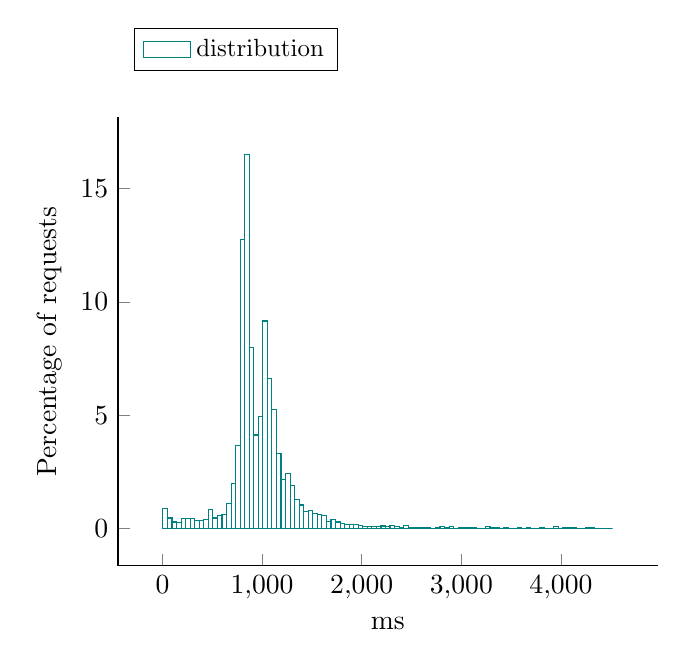
\begin{tikzpicture}
            \begin{axis}[ylabel = Percentage of requests, 
xlabel = ms, 
legend style = {nodes={scale=0.9, transform shape}, at={(0.03,1.2)}, anchor=north west, draw=black, fill=white, align=left, legend columns=3},
area style, mark size = 0pt,
 cycle list name = exotic,
  axis lines* = left]
		\addplot +[ybar interval] coordinates {
			 (5, 0.875657)
			 (50.59, 0.453281)
			 (96.18, 0.27815)
			 (141.77, 0.236942)
			 (187.36, 0.442979)
			 (232.95, 0.432677)
			 (278.54, 0.422376)
			 (324.13, 0.339961)
			 (369.72, 0.350263)
			 (415.31, 0.401772)
			 (460.9, 0.834449)
			 (506.49, 0.453281)
			 (552.08, 0.545998)
			 (597.67, 0.618111)
			 (643.26, 1.092)
			 (688.85, 1.98826)
			 (734.44, 3.66746)
			 (780.03, 12.764)
			 (825.62, 16.5036)
			 (871.21, 8.00453)
			 (916.8, 4.12074)
			 (962.39, 4.93458)
			 (1007.98, 9.15834)
			 (1053.57, 6.62409)
			 (1099.16, 5.25394)
			 (1144.75, 3.28629)
			 (1190.34, 2.16339)
			 (1235.93, 2.41063)
			 (1281.52, 1.89554)
			 (1327.11, 1.25682)
			 (1372.7, 1.03018)
			 (1418.29, 0.752035)
			 (1463.88, 0.78294)
			 (1509.47, 0.66962)
			 (1555.06, 0.607809)
			 (1600.65, 0.5563)
			 (1646.24, 0.319357)
			 (1691.83, 0.39147)
			 (1737.42, 0.27815)
			 (1783.01, 0.216339)
			 (1828.6, 0.154528)
			 (1874.19, 0.175131)
			 (1919.78, 0.185433)
			 (1965.37, 0.123622)
			 (2010.96, 0.0618111)
			 (2056.55, 0.0927166)
			 (2102.14, 0.0824148)
			 (2147.73, 0.0618111)
			 (2193.32, 0.103018)
			 (2238.91, 0.0618111)
			 (2284.5, 0.11332)
			 (2330.09, 0.0618111)
			 (2375.68, 0.0515092)
			 (2421.27, 0.11332)
			 (2466.86, 0.0206037)
			 (2512.45, 0.0515092)
			 (2558.04, 0.0412074)
			 (2603.63, 0.0515092)
			 (2649.22, 0.0412074)
			 (2694.81, 0.0103018)
			 (2740.4, 0.0412074)
			 (2785.99, 0.0721129)
			 (2831.58, 0.0206037)
			 (2877.17, 0.0618111)
			 (2922.76, 0.0103018)
			 (2968.35, 0.0206037)
			 (3013.94, 0.0412074)
			 (3059.53, 0.0309055)
			 (3105.12, 0.0309055)
			 (3150.71, 0)
			 (3196.3, 0)
			 (3241.89, 0.0824148)
			 (3287.48, 0.0412074)
			 (3333.07, 0.0206037)
			 (3378.66, 0)
			 (3424.25, 0.0309055)
			 (3469.84, 0.0103018)
			 (3515.43, 0.0103018)
			 (3561.02, 0.0206037)
			 (3606.61, 0)
			 (3652.2, 0.0206037)
			 (3697.79, 0)
			 (3743.38, 0)
			 (3788.97, 0.0309055)
			 (3834.56, 0.0103018)
			 (3880.15, 0.0103018)
			 (3925.74, 0.0721129)
			 (3971.33, 0.0103018)
			 (4016.92, 0.0206037)
			 (4062.51, 0.0309055)
			 (4108.1, 0.0515092)
			 (4153.69, 0)
			 (4199.28, 0.0103018)
			 (4244.87, 0.0515092)
			 (4290.46, 0.0206037)
			 (4336.05, 0)
			 (4381.64, 0.0103018)
			 (4427.23, 0.0103018)
			 (4472.82, 0)
			 (4518.41, 0.0103018)
		};
\addlegendentry{distribution};
           \end{axis}
      \end{tikzpicture}
  \end{adjustbox}
  \caption{Response time distribution - req = ReadUser-3}
\end{figure}
\end{minipage}\hfill\begin{minipage}{0.18\linewidth}
\begin{table}[h]
\begin{tabular}{|cc|}
\hline
\textbf{} & \textbf{ms}\\ \hline
 \Xhline{0.005\arrayrulewidth}
min & 5\\
 \Xhline{0.005\arrayrulewidth}
max & 4564\\
 \Xhline{0.005\arrayrulewidth}
mean & 989\\
 \Xhline{0.005\arrayrulewidth}
std & 395\\
\hline
\hline
 \Xhline{0.005\arrayrulewidth}
25th & 822\\
 \Xhline{0.005\arrayrulewidth}
50th & 911\\
 \Xhline{0.005\arrayrulewidth}
75th & 1096\\
 \Xhline{0.005\arrayrulewidth}
80th & 1138\\
 \Xhline{0.005\arrayrulewidth}
85th & 1211\\
 \Xhline{0.005\arrayrulewidth}
90th & 1308\\
 \Xhline{0.005\arrayrulewidth}
95th & 1549\\
 \Xhline{0.005\arrayrulewidth}
99th & 2627\\
\hline
\end{tabular}
\caption{Response time}
\end{table}
\end{minipage}\hfill